	\chapter*{Introduction}
	Dans une entreprise, il y a 6 ressources : 
	\begin{itemize}
		\item Humaines
		\item Recherche et développement
		\item Production 
		\item Commerciale
		\item Finances 
		\item Information
	\end{itemize}

	Chacune de ces ressources à un directeur\footnote{Directeur commercial, Directeur
	Ressources humains, Directeur financier, \ldots}, ici nous aborderons principalement
	les ressources humaines.
	
	\chapter{Réussir un entretien}

	En arrivant dans une entreprise on demande un projet, à distinguer avec un
	objectif\footnote{Exemple d'objectif, devenir ingénieur développement}, un projet est
	lié à la motivation : << qu'est ce que j'ai envie de faire ? >>, afin d'être pris au
	sérieux il faut donc dire ce qu'on veut faire, ce qu'on va apporter à
	l'entreprise.

	Afin d'effectuer une bonne carrière, deux compétences sont très importantes: 
	\begin{description}
		\item[Communication] Clients, Hiérarchie, \ldots
		\item[Négociation] Salaires, postes, clients, \ldots
		\item[Management] Gérer une équipe, motiver les gens, les faire collaborer, donner envie de travailler,\ldots
	\end{description}

	Évaluation des compétences : 
	\begin{description}
		\item[Savoir] Diplôme
		\item[Savoir faire] Expérience
		\item[Savoir être] Attitudes générale
	\end{description}

	\chapter{Les ressources humaines}
	Les ressources humaines sont là pour gérer le personnel, elles doivent aider à faire avancer le personnel.

	Chaque personne de l'entreprise à du potentiel : Avoir des compétences mais aussi de la motivation. 

	Les ressources humaines sont là pour que le plus de personnes ai le maximum de résultats, avec une bonne rh, personne ne doit se retrouver en bas à
	gauche.

	\begin{figure}[H]
		\centering
		\includegraphics[width=5cm]{figure1.eps}
	\end{figure}
	Une entreprise doit avoir beaucoup d'espoirs et pilliers, éviter trop d'étoiles, pour éviter les conflits.

	\section{Objectifs d'un DRH}
	\begin{description}
		\item[Abaisser les effectifs] préférer enrichir les postes des utilisateurs
		\item[Abaisser la masse salariale] Réduire les échelons, utiliser des logiciels de gestion, \ldots
		\item[Multiplier les compétences] 
	\end{description}

	\section{Finalité de la RH}
	\subsection{Recruter}
	Travailler avec la hiérarchie pour décrire le post, trouver les compétences nécessaire et vont chercher les profils nécessaires.
	\begin{remarque}
		Pour une candidature spontanée, ils est préférable de contacter le directeur du service plutôt que la RH: les RH auront une approche qui
		concerne plus la gestion de l'entreprise(pyramides des ages, diplômes, experience, \ldots) alors que le service regardera les compétences.
	\end{remarque}

	\subsection{Former}
	La formation interne à l'entreprise : faire en sorte que l'entreprise ai les compétences nécessaires au bon moment.

	\subsection{Gérer}
	Gérer les effectifs\footnote{savoir combien il y a de personnes qui travaillent à un instant T}, les congés, les RTT, les crédits formations.
	
	\subsection{Administration}
	Suivis administratif des gens : faire évoluer leur état civil, coefficient en fonction du poste, \ldots

	\subsection{Négocier}
	Obligation de négocier tous le ans avec les syndicats.(Sans obligation d'aboutissement) 

	\subsection{Organiser}
	Organisation du travail optimal.

	\subsection{Communication}
	Deux types : externe et interne. 

	Plusieurs types de communication : papier (journaux d'entreprise, courriers, \ldots) dite formel et une communication informelle par mail, internet,
	\ldots


	

